%!TEX root = ../thesis.tex
% ******************************* Thesis Appendix B ****************************
\chapter{Supporting work for \autoref*{chap:dst}}

% =======================================
\section{Full drug susceptibility data available}
\label{sec:full-dst}

Available phenotype information for culture-based \emph{and} line probe assay (LPA) drug susceptibility testing (DST) are shown in \autoref{tab:full-dst} and \autoref{fig:full-dst}.

\begin{table}
\centering
\begin{tabular}{|l|c|}
\hline
Drug              & Count \\ \hline
Amikacin          & 88    \\ \hline
Amikacin-LPA      & 30    \\ \hline
Capreomycin       & 51    \\ \hline
Capreomycin-LPA   & 27    \\ \hline
Ciprofloxacin-LPA & 5     \\ \hline
Ethambutol        & 90    \\ \hline
Ethambutol-LPA    & 21    \\ \hline
Isoniazid         & 98    \\ \hline
Isoniazid-LPA     & 124   \\ \hline
Kanamycin         & 51    \\ \hline
Kanamycin-LPA     & 27    \\ \hline
Moxifloxacin      & 1     \\ \hline
Moxifloxacin-LPA  & 5     \\ \hline
Ofloxacin         & 86    \\ \hline
Ofloxacin-LPA     & 30    \\ \hline
Pyrazinamide      & 1     \\ \hline
Rifampicin        & 91    \\ \hline
Rifampicin-LPA    & 124   \\ \hline
Streptomycin      & 90    \\ \hline
\end{tabular}
\caption{Culture-based and line probe assay (LPA) drug susceptibility data available for samples. The counts are the number of samples with phenotype information available for that drug.}
\label{tab:full-dst}
\end{table}

\begin{figure}
\begin{center}
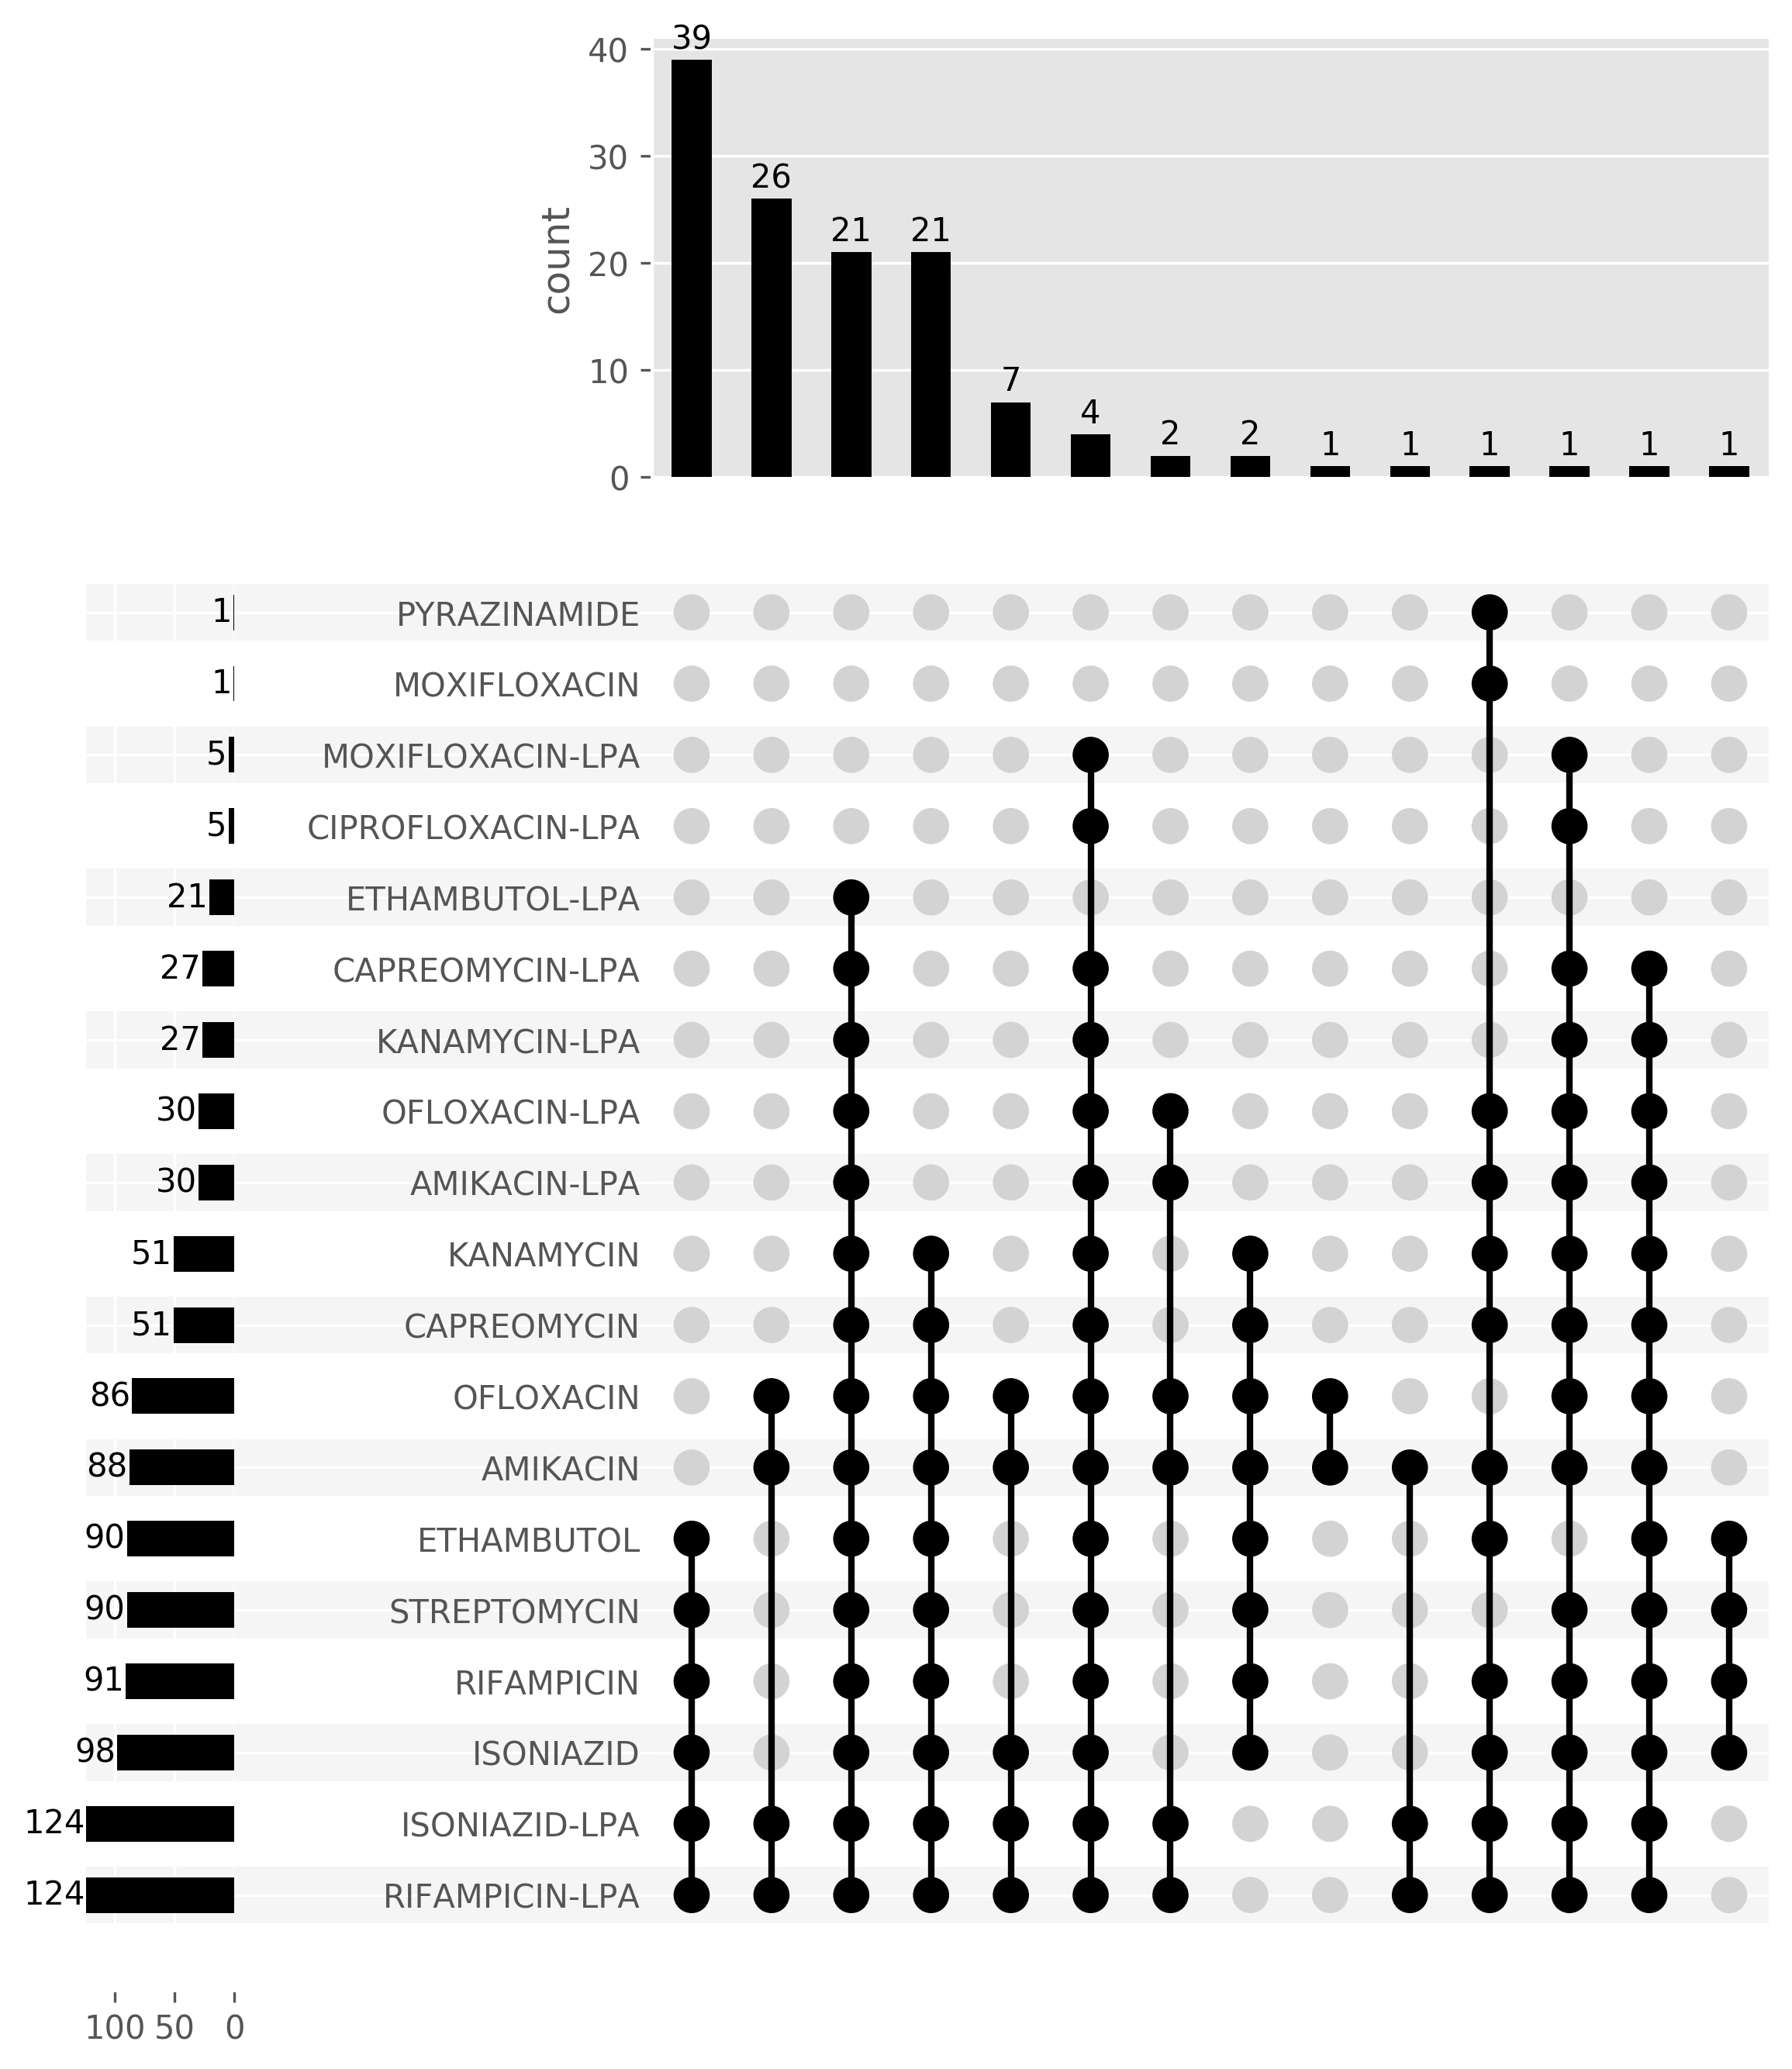
\includegraphics[width=0.90\columnwidth]{Appendix2/Figs/full-available-dst.png}
\caption{{Culture-based and line probe assay (LPA) drug susceptibility data available for samples. Each row is a drug, and the columns represent a set of samples that have phenotype information for those drugs with a filled cell. The top panel shows the number of samples in the set for that combination of drugs. The bar plot in the left panel shows the number of samples with phenotype information for that drug.
{\label{fig:full-dst}}
}}
\end{center}
\end{figure}